\chapter{Felhasználói dokumentáció}
\label{ch:user}

A szoftvernek két felhasználói felülete van: 
egy parancssoros felhasználói felület (CLI - command line interface) 
az adathalmaz generálásához és 
egy grafikus felhasználói felület (GUI - graphical user interface) 
az átalakítások szemléltetéséhez és az adathalmaz böngészéséhez. 
Mindkét felhasználói felület nyelve angol.

\section{Futtatási környezet}

Az alkalmazás egy Python 3.10-es vagy újabb verziójú Python interpreterrel futtatható.
A futtatáshoz az alakalmazás függőségeit installálni kell a pip csomagkezelővel.
A függőségek a projekt mappában a \emph{requirements.txt} fájlban találhatók, 
és a következő paranccsal installálhatók:
\begin{lstlisting}
$ pip install -r requirements.txt
\end{lstlisting}

\section{Adatbázis beállítása}
Az alkalmazás működéséhez sükség van egy elérhető \emph{mongodb} adatbázisra.
Ezt a projekt \emph{config} könyvtárában található \emph{default.ini} konfigfájlban lehet beállítani.

Három paraméter szükséges:
\begin{itemize}
	\item \emph{host} - host neve (URL), pl.: localhost
	\item \emph{port} - port száma (egész), pl.: 27017
	\item \emph{database} - adatbázis neve
\end{itemize}

\section{Adathalmazt generáló CLI}

Ezzel a CLI alkalmazással van lehetőségünk egy adathalmaz generálására.

\subsection{Alkalmazás használata}

Az alkalmazás a projekt könyvtárból indítható a következő paranccsal:

\begin{lstlisting}
$ python -m source.persistor <mode> <path>
\end{lstlisting}

Két paraméter szükséges:
\begin{enumerate}
	\item\label{step:first} \emph{mode} - az adatok forrásának típusa,
	lehetséges értékek:
	\begin{itemize}
		\item \emph{csv} - csv fájlból olvassa a forrásfájlok tartalmát
		\item \emph{dir} - könyvtárból rekurzívan olvassa a forrásfájlokat
	\end{itemize}
	\item \emph{path} - az adatok forrásának elérési útvonala, 
	csv olvasása esetén a forráskódok csak az első oszlopban lehetnek
\end{enumerate}

\begin{figure}[H]
	\centering
	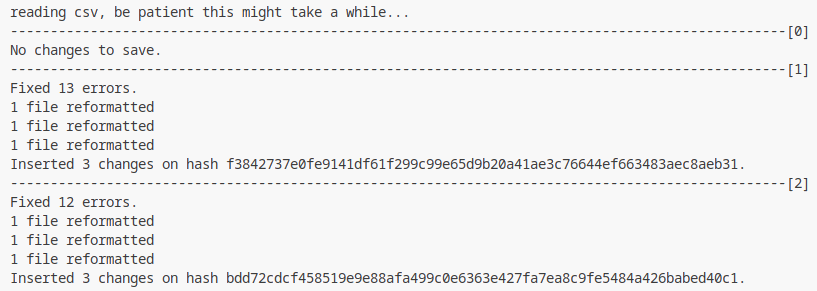
\includegraphics[width=0.8\textwidth,frame]{log}
	\caption{A program a kiírja a feldolgozott fájllal kapcsolatos adatokat.}
\end{figure}

\section{Átalakításokat szemléltető GUI}

Ez a GUI alkamazás szemlélteti az átalakításokat. 
Kipróbálhatunk vele egy vagy több átalakítást, vizualizáhatjuk kódok absztrakt szintaxis fáját, 
és az adatbázisba bekerült átalakítások eredményét is megnézhetjük.

\section{Képek, ábrák}

Aliquam vehicula luctus mi a pretium. Nulla quam neque, maximus nec velit in, aliquam mollis tortor. Aliquam erat volutpat. Curabitur vitae laoreet turpis. Integer id diam ligula. Nulla sodales purus id mi consequat, eu venenatis odio pharetra. Cras a arcu quam. Suspendisse augue risus, pulvinar a turpis et, commodo aliquet turpis. Nulla aliquam scelerisque mi eget pharetra. Mauris sed posuere elit, ac lobortis metus. Proin lacinia sit amet diam sed auctor. Nam viverra orci id sapien sollicitudin, a aliquam lacus suscipit, \ref{fig:example-1}.~ábra:

\begin{figure}[H]
	\centering
	
\includegraphics[width=0.6\textwidth,height=100px]{elte_cimer_szines}
	\caption{Quisque ac tincidunt leo}
	\label{fig:example-1}
\end{figure}

\subsection{Képek szegélyezése}

Ut aliquet nec neque eget fermentum. Cras volutpat tellus sed placerat elementum. Quisque neque dui, consectetur nec finibus eget, blandit id purus. Nam eget ipsum non nunc placerat interdum.

\begin{figure}[H]
	\centering
	
\includegraphics[width=0.6\textwidth,height=100px,frame]{elte_cimer_szines}
	\caption{Quisque ac tincidunt leo}
\end{figure}

\subsection{Képek csoportosítása}

In non ipsum fermentum urna feugiat rutrum a at odio. Pellentesque habitant morbi tristique senectus et netus et malesuada fames ac turpis egestas. Nulla tincidunt mattis nisl id suscipit. Sed bibendum ac felis sed volutpat. Nam pharetra nisi nec facilisis faucibus. Aenean tristique nec libero non commodo. Nulla egestas laoreet tempus. Nunc eu aliquet nulla, quis vehicula dui. Proin ac risus sodales, gravida nisi vitae, efficitur neque, \ref{fig:example-2}.~ábra:

\begin{figure}[H]
	\centering
	\subcaptionbox{Vestibulum quis mattis urna}{
		
\includegraphics[width=0.45\linewidth]{elte_cimer_szines}}
	\hspace{5pt}
	\subcaptionbox{Donec hendrerit quis dui sit amet venenatis}{
		
\includegraphics[width=0.45\linewidth]{elte_cimer_szines}}
	\caption{Aenean porttitor mi volutpat massa gravida}
	\label{fig:example-2}
\end{figure}

Nam et nunc eget elit tincidunt sollicitudin. Quisque ligula ipsum, tempor vitae tortor ut, commodo rhoncus diam. Pellentesque habitant morbi tristique senectus et netus et malesuada fames ac turpis egestas. Phasellus vehicula quam dui, eu convallis metus porta ac.


\section{Táblázatok}

Nam magna ex, euismod nec interdum sed, sagittis nec leo. Nam blandit massa bibendum mattis tristique. Phasellus tortor ligula, sodales a consectetur vitae, placerat vitae dolor. Aenean consequat in quam ac mollis. 

\begin{table}[H]
	\centering
	\begin{tabular}{ | m{0.25\textwidth} | m{0.65\textwidth} | }
		\hline
		\textbf{Phasellus tortor} & \textbf{Aenean consequat} \\
		\hline \hline
		\emph{Sed malesuada} & Aliquam aliquam velit in convallis ultrices. \\
		\hline
		\emph{Purus sagittis} &  Quisque lobortis eros vitae urna lacinia euismod. \\
		\hline
		\emph{Pellentesque} & Curabitur ac lacus pellentesque, eleifend sem ut, placerat enim. Ut auctor tempor odio ut dapibus. \\
		\hline
	\end{tabular}
	\caption{Maecenas tincidunt non justo quis accumsan}
	\label{tab:example-1}
\end{table}

\subsection{Sorok és oszlopok egyesítése}

Mauris a dapibus lectus. Vestibulum commodo nibh ante, ut maximus magna eleifend vel. Integer vehicula elit non lacus lacinia, vitae porttitor dolor ultrices. Vivamus gravida faucibus efficitur. Ut non erat quis arcu vehicula lacinia. Nulla felis mauris, laoreet sed malesuada in, euismod et lacus. Aenean at finibus ipsum. Pellentesque dignissim elit sit amet lacus congue vulputate.

\begin{table}[htb]
	\centering
	\begin{tabular}{ | c | r | r | r | r | r | r | }
		\hline
		\multirow{2}{*}{\textbf{Quisque}} & \multicolumn{2}{ c | }{\textbf{Suspendisse}} & \multicolumn{2}{ c | }{\textbf{Aliquam}} & \multicolumn{2}{ c | }{\textbf{Vivamus}} \\
		\cline{2-7}
		& Proin & Nunc & Proin & Nunc & Proin & Nunc \\
		\hline \hline		
		Leo & 2,80 MB & 100\% & 232 KB & 8,09\% & 248 KB & 8,64\% \\
		\hline
		Vel & 9,60 MB & 100\% & 564 KB & 5,74\% & 292 KB & 2,97\% \\
		\hline
		Auge & 78,2 MB & 100\% & 52,3 MB & 66,88\% & 3,22 MB & 4,12\% \\
		\hline 
	\end{tabular}
	\caption[Rövid cím a táblázatjegyzékbe]{Vivamus ac arcu fringilla, fermentum neque sed, interdum erat. Mauris bibendum mauris vitae enim mollis, et eleifend turpis aliquet.}
	\label{tab:example-2}
\end{table}

\subsection{Több oldalra átnyúló táblázatok}

Nunc porta placerat leo, sit amet porttitor dui porta molestie. Aliquam at fermentum mi. Maecenas vitae lorem at leo tincidunt volutpat at nec tortor. Vivamus semper lacus eu diam laoreet congue. Vivamus in ipsum risus. Nulla ullamcorper finibus mauris non aliquet. Vivamus elementum rhoncus ex ut porttitor.

\begin{center}
	\begin{longtable}{ | p{0.3\textwidth} | p{0.7\textwidth} | }
		
		\hline
		\multicolumn{2}{|c|}{\textbf{Praesent aliquam mauris enim}}
		\\ \hline
		
		\emph{Suspendisse potenti} & \emph{Lorem ipsum dolor sit amet}
		\\ \hline \hline
		\endfirsthead % első oldal fejléce
		
		\hline
		\emph{Suspendisse potenti} & \emph{Lorem ipsum dolor sit amet}
		\\ \hline \hline
		\endhead % többi oldal fejléce
		
		\hline
		\endfoot % többi oldal lábléce
		
		\endlastfoot % utolsó oldal lábléce
		
		\emph{Praesent}
		& Nulla ultrices et libero sit amet fringilla. Nunc scelerisque ante tempus sapien placerat convallis.
		\\ \hline
		
		\emph{Luctus}
		& Integer hendrerit erat massa, non hendrerit risus convallis at. Curabitur ultrices, justo in imperdiet condimentum, neque tortor luctus enim, luctus posuere massa erat vitae nibh.
		\\ \hline
		
		\emph{Egestas}
		& Duis fermentum feugiat augue in blandit. Mauris a tempor felis. Pellentesque ultricies tristique dignissim. Pellentesque aliquam semper tristique. Nam nec egestas dolor. Vestibulum id elit quis enim fringilla tempor eu a mauris. Aliquam vitae lacus tellus. Phasellus mauris lectus, aliquam id leo eget, auctor dapibus magna. Fusce lacinia felis ac elit luctus luctus.
		\\ \hline
		
		\emph{Dignissim}
		& Praesent aliquam mauris enim, vestibulum posuere massa facilisis in. Suspendisse potenti. Nam quam purus, rutrum eu augue ut, varius vehicula tellus. Fusce dui diam, aliquet sit amet eros at, sollicitudin facilisis quam. Phasellus tempor metus vel augue gravida pretium. Proin aliquam aliquam blandit. Nulla id tempus mi. Fusce in aliquam tortor.
		\\ \hline
		
		\emph{Pellentesque}
		& Donec felis nibh, imperdiet a arcu non, vehicula gravida nibh. Quisque interdum sapien eu massa commodo, ac elementum felis faucibus.
		\\ \hline
		
		\emph{Molestie}
		& Cras ullamcorper tellus et auctor ultricies. Maecenas tincidunt euismod lectus nec venenatis. Suspendisse potenti. Pellentesque pretium nunc ut euismod cursus. Nam venenatis condimentum quam. Curabitur suscipit efficitur aliquet. Interdum et malesuada fames ac ante ipsum primis in faucibus.
		\\ \hline
		
		\emph{Vivamus semper}
		& In purus purus, faucibus eu libero vulputate, tristique sodales nunc. Nulla ut gravida dolor. Fusce vel pellentesque mi, vel efficitur eros. Nunc vitae elit tellus. Sed vestibulum auctor consequat. 
		\\ \hline
		
		\emph{Condimentum}
		& Nulla scelerisque, leo et facilisis pretium, risus enim cursus turpis, eu suscipit ipsum ipsum in mauris. Praesent eget pulvinar ipsum, suscipit interdum nunc. Nam varius massa ut justo ullamcorper sollicitudin. Vivamus facilisis suscipit neque, eu fermentum risus. Ut at mi mauris.
		\\ \hline
		
		\caption{Praesent ullamcorper consequat tellus ut eleifend}
		\label{tab:example-3}		
	\end{longtable}
\end{center}